\documentclass[border=5pt]{standalone}
\usepackage{tikz}
\usetikzlibrary{positioning, arrows.meta}

\definecolor{servercolor}{RGB}{86, 163, 239}
\definecolor{clientcolor}{RGB}{239, 123, 86}
\definecolor{errorcolor}{RGB}{220, 53, 69}
\definecolor{correctcolor}{RGB}{40, 167, 69}
\definecolor{labelbg}{RGB}{248, 249, 250}
\definecolor{codebg}{RGB}{243, 243, 243}

\begin{document}
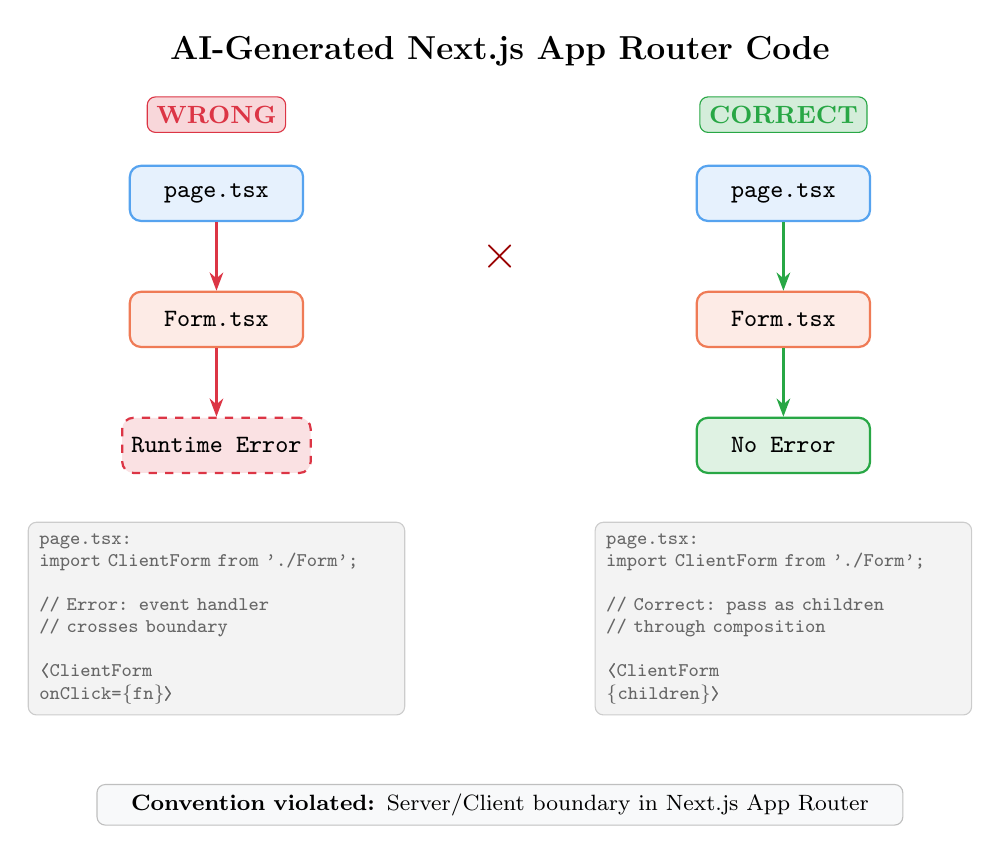
\begin{tikzpicture}[
    node distance=0.8cm and 2.6cm,
    box/.style={draw, rounded corners=4pt, minimum width=2.2cm, minimum height=0.7cm, align=center, font=\ttfamily\small},
    server/.style={box, fill=servercolor!15, draw=servercolor, thick},
    client/.style={box, fill=clientcolor!15, draw=clientcolor, thick},
    error/.style={box, fill=errorcolor!15, draw=errorcolor, thick, dashed},
    ok/.style={box, fill=correctcolor!15, draw=correctcolor, thick},
    code/.style={rectangle, draw=black!20, fill=codebg, rounded corners=3pt, inner sep=4pt, font=\ttfamily\scriptsize, text=black!60, align=left},
    arrow/.style={->, >=Stealth, thick}
]

% Title
\node[font=\large\bfseries] at (0, 0) {AI-Generated Next.js App Router Code};

% ============ LEFT: WRONG ============
\node[fill=errorcolor!20, draw=errorcolor, rounded corners=3pt, font=\small\bfseries, text=errorcolor] (wrong-badge) at (-3.6, -0.8) {WRONG};
\node[server] (server-w) at (-3.6, -1.8) {page.tsx};
\node[client] (client-w) at (-3.6, -3.4) {Form.tsx};
\node[error] (error-w) at (-3.6, -5.0) {Runtime Error};

\node[code, text width=4.5cm, minimum height=2.0cm] (wrongcode) at (-3.6, -7.2) {%
\textbf{page.tsx:}\newline
import ClientForm from './Form';\newline\newline
// Error: event handler\newline
// crosses boundary\newline\newline
\textlangle ClientForm\newline
  onClick=\{fn\}\textrangle
};

\draw[arrow, errorcolor] (server-w) -- (client-w);
\draw[arrow, errorcolor] (client-w) -- (error-w);

% ============ DIVIDER ============
\node[font=\LARGE\bfseries, text=red!60!black] at (0, -2.6) {$\times$};

% ============ RIGHT: CORRECT ============
\node[fill=correctcolor!20, draw=correctcolor, rounded corners=3pt, font=\small\bfseries, text=correctcolor] (right-badge) at (3.6, -0.8) {CORRECT};
\node[server] (server-r) at (3.6, -1.8) {page.tsx};
\node[client] (client-r) at (3.6, -3.4) {Form.tsx};
\node[ok] (ok-r) at (3.6, -5.0) {No Error};

\node[code, text width=4.5cm, minimum height=2.0cm] (rightcode) at (3.6, -7.2) {%
\textbf{page.tsx:}\newline
import ClientForm from './Form';\newline\newline
// Correct: pass as children\newline
// through composition\newline\newline
\textlangle ClientForm\newline
  \{children\}\textrangle
};

\draw[arrow, correctcolor] (server-r) -- (client-r);
\draw[arrow, correctcolor] (client-r) -- (ok-r);

% Bottom legend
\node[below=0.1cm of wrongcode, fill=labelbg, draw=gray!50, rounded corners=3pt, font=\footnotesize, text width=10cm, align=center] at (0, -9.2) {%
\textbf{Convention violated:} Server/Client boundary in Next.js App Router
};

\end{tikzpicture}
\end{document}
